Im Folgenden sind die während des Versuchs aufgenommenen Messwerte tabellarisch dargestellt.
Da die selbst berechneten Fourierkoeffizienten zu Beginn des Versuchs noch Fehler 
aufwiesen, wurden für die Versuchsdurchführung folgende Fourierkoeffizienten verwendet.

\begin{subequations}
	\begin{empheq}{align}
	\label{eq:Koeff_Recht}
	\text{Rechteck:}\qquad b_{n} &= \dfrac{4A}{n\pi}\quad, n\mod{2} \neq 0 \\
	\label{eq:Koeff_Drei}
	\text{Dreieck:}\qquad		b_{n} &= \dfrac{4A}{(n\pi)^{2}}\quad, n\mod{2} \neq 0\\
	\label{eq:Koeff_Säge}
	\text{Sägezahn:}\qquad		b_{n} &= \dfrac{2A}{n\pi}\quad, \forall n
	\end{empheq}
\end{subequations}

   
\newpage
\subsection{Fourier-Analyse}\label{sec:Auswertung_Analyse}
In \cref{tab:Analyse1} befinden sich sowohl die im Versuch gemessenen, 
als auch die aus den 
Koeffizienten \cref{eq:Koeff_Recht} bis \cref{eq:Koeff_Säge} berechneten Amplituden der ersten 
Oberschwingungen, aus denen sich das jeweilige Signal mit der Frequenz $\nu_{1} = \SI{100}{\hertz}$ 
und der Amplitude $\hat{U} = \SI{2}{\volt}$ zusammensetzt. 
  
  

\begin{table}[!h]
	\centering
	\begin{tabular}{|c|c|c|c|}
		\hline
		Frequenzen & Gemessene Amplitude & Berechnete Amplitude & relative Abweichung \\ 
		$\nu\,[\si{\hertz}]$ & $b_{n}\,[\si{\volt}]$ & $b_{n,theo}\,[\si{\volt}]$ & $\envert{1 - \tfrac{b_{n}}{b_{n,theo}}}$  \\\hline\hline
		\num{100}  & \num{1.80}  & \num{2.55}  & \num{0.29}  \\ 
		\num{300}  & \num{0.60}  & \num{0.85}  & \num{0.29}  \\ 
		\num{500}  & \num{0.34} & \num{0.51}  & \num{0.33} \\
		\num{700}  & \num{0.25} & \num{0.36}  & \num{0.31} \\ 
		\num{900}  & \num{0.19} & \num{0.28}  & \num{0.32} \\ 
		\num{1100} & \num{0.14} & \num{0.23}  & \num{0.39} \\\hline
	\end{tabular}
	\caption{Gemessene und Berechnete Amplituden der Oberschwingung\\ \hspace*{2.1cm}und deren relative Abweichung für die Rechteckspannung \label{tab:Analyse1}}
\end{table}

\begin{table}[!h]
	\centering
	\begin{tabular}{|c|c|c|c|}
		\hline
		Frequenzen & Gemessene Amplitude & Berechnete Amplitude & relative Abweichung\\
		$\nu\,[\si{\hertz}]$ & $b_{n}\,[\si{\volt}]$ & $b_{n,theo}\,[\si{\volt}]$& $\envert{1 - \tfrac{b_{n}}{b_{n,theo}}}$ \\\hline\hline
		\num{100}  & \num{1.16}  & \num{0.80} & \num{0.43}\\
		\num{300}  & \num{0.16}  & \num{0.09} & \num{0.78}\\
		\num{500}  & \num{0.08}  & \num{0.03} & \num{1.47}\\
		\num{700}  & \num{0.05}  & \num{0.02} & \num{1.78}\\
		\num{900}  &\num{0.04}  & \num{0.01} & \num{3.00}\\
		\hline
	\end{tabular}
	\caption{Gemessene und Berechnete Amplituden der Oberschwingung\\ \hspace*{2.1cm}und deren relative Abweichung für die Dreiecksspannung \label{tab:Analyse2}}
\end{table}		
\begin{table}[!h]
	\centering
	\begin{tabular}{|c|c|c|c|}
		\hline
		Frequenzen & Gemessene Amplitude & Berechnete Amplitude & relative Abweichung\\
		$\nu\,[\si{\hertz}]$ & $b_{n}\,[\si{\volt}]$ & $b_{n}\,[\si{\volt}]$ & $\envert{1 - \tfrac{b_{n}}{b_{n,theo}}}$\\\hline\hline
		\num{100}  & \num{0.88}  & \num{0.880}  & \num{0.00} \\
		\num{200}  & \num{0.45}  & \num{0.440}  & \num{0.02} \\
		\num{300}  & \num{0.29}  & \num{0.293}  & \num{0.01} \\
		\num{400}  & \num{0.24}  & \num{0.220}  & \num{0.07} \\
		\num{500}  & \num{0.20}  & \num{0.176}  & \num{0.14} \\
		\num{600}  & \num{0.15}  & \num{0.147}  & \num{0.01} \\
		\num{700}  & \num{0.12}  & \num{0.126}  & \num{0.05} \\
		\hline
	\end{tabular}
	\caption{Gemessene und Berechnete Amplituden der Oberschwingung der Sägezahnspannung \label{tab:Analyse3}}
\end{table}



\subsection{Fourier-Synthese}\label{sec:Auswertung_Synthese}

Die für die Fourier-Synthese benötigten Amplituden wurden aus den Koeffizienten \cref{eq:Koeff_Recht} bis \cref{eq:Koeff_Säge}
bestimmt. Wobei die folgenden Koeffizienten der zu erzeugenden Spannung jeweils aus 
der Amplitude des Koeffizienten der ersten Oberwelle $A_{1} = \SI{0.8}{\volt}$
berechnet wurden, diese sind in 
%Die Berechnung sei beispielhaft an der Rechteckspannung gezeigt:   
%\begin{empheq}{align*}
%	b_{n} &= \dfrac{4A_{r}}{n\pi}\ ,\ n = 1\\
%	b_{1}&= \dfrac{4A_{r}}{\pi}\\
%	A_{r} &= b_{1}\dfrac{\pi}{4}\ , \ b_{1} = \SI{0.8}{\volt} \\
%	A_{r} &= \SI{0.2}{\volt}\cdot\pi
%\end{empheq}
%
%Damit ergeben sich die Amplituden $A$ der Koeffizienten zu:
%  \begin{subequations}
%  	\begin{empheq}{align*}
%  	\text{Rechteck:}\qquad A_{r} &= \SI{0.2}{\volt} \cdot \pi \\
%  	\text{Dreieck:}\qquad  A_{d} &= \SI{0.2}{\volt} \cdot \pi^{2}\\
%  	\text{Sägezahn:}\qquad A_{s} &= \SI{0.4}{\volt} \cdot \pi
%  	\end{empheq}
%  \end{subequations}
sind in \cref{tab:Synthese} zu finden, wobei nicht auftretende
Amplituden durch \enquote{-} dargestellt sind. 

\begin{table}[!h]
	\centering
	\begin{tabular}{|c|c|c|}
		\hline
		  Rechteck Amplitude    &    Dreieck Amplitude    &   Sägezahn Amplitude    \\
		$b_{n,r}\,[\si{\volt}]$ & $b_{n,d}\,[\si{\volt}]$ & $b_{n,s}\,[\si{\volt}]$ \\ \hline\hline
		      \num{0.80}        &       \num{0.80}        &       \num{0.80}        \\
		           -            &            -            &       \num{0.40}        \\
		      \num{0.34}        &       \num{0.09}        &       \num{0.27}        \\
		           -            &            -            &       \num{0.20}        \\
		      \num{0.20}        &       \num{0.03}        &       \num{0.16}        \\
		           -            &            -            &       \num{0.13}        \\
		      \num{0.15}        &       \num{0.02}        &       \num{0.11}        \\
		           -            &            -            &       \num{0.10}        \\
		      \num{0.11}        &       \num{0.01}        &       \num{0.09}        \\
		           -            &            -            &       \num{0.08}        \\ \hline
	\end{tabular}
	\caption{Zur Synthese verwandte Amplituden der ersten 10 Oberwellen \label{tab:Synthese}}
\end{table}  

Durch Einstellen der Amplituden aus \cref{tab:Synthese} und der Phasen zwischen den Oberwellen am Oberwellengenerator
erhält man die in \crefrange{fig:Recht}{fig:Säge} dargestellten Spannungsverläufe.

\begin{figure}[h!]
	\centering
	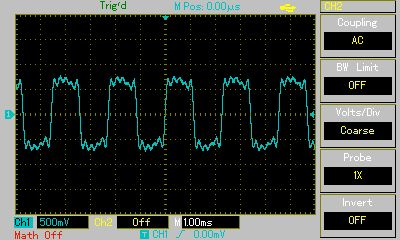
\includegraphics[scale=0.8]{Grafiken/Rechteckspannung.jpg}
	\caption{Synthetisierte Rechteckspannung}
	\label{fig:Recht}
\end{figure}

\begin{figure}[h!]
	\centering
	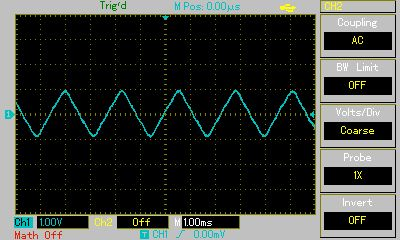
\includegraphics[scale=0.8]{Grafiken/Dreieckspannung.jpg}
	\caption{Synthetisierte Dreieckspannung}
	\label{fig:Drei}
\end{figure}

\begin{figure}[h!]
	\centering
	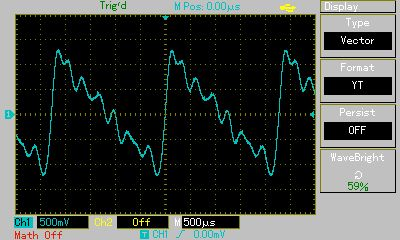
\includegraphics[scale=0.8]{Grafiken/Saegezahnspannung.jpg}
	\caption{Synthetisierte Sägezahnspannung}	
	\label{fig:Säge}
\end{figure}
\hspace*{4cm}